\documentclass[9pt,twocolumn,twoside]{../../styles/osajnl}
\usepackage{fancyvrb}
\journal{i524}

\title{An Overview of Pivotal HD/HAWQ and its Applications}

%\author[1,2,3]{John Smith}
%\author[2]{Alice Smith}
%\author[1]{Bruce Wayne}
\author[1]{Veera Marni}

\affil[1]{School of Informatics and Computing, Bloomington, IN 47408, U.S.A.}
%\affil[2]{School of Science, University of Technology, 2000 J St. NW, Washington DC, 20036}
%\affil[3]{School of Optics, University of Technology, 2000 J St. NW, Washington DC, 20036}

\affil[*]{Corresponding authors: vmarni@umail.iu.edu}

%\dates{project-000, \today}
\dates{\today}

\ociscodes{pivotal, hd, hawq, data science}

% replace this with your url in github/gitlab
\doi{\url{https://github.com/narayana1043/sp17-i524/blob/master/paper2/S17-IR-2017/report.pdf}}


\begin{abstract}
 Pivotal HD/HAWQ is a Hadoop native SQL query engine that combines
 the key technological advantages of MPP database with the
 scalability and convenience of Hadoop. \newline
\end{abstract}

\setboolean{displaycopyright}{true}

\begin{document}

\maketitle
\TODO{This review document is provided for you to achieve your
  best. We have listed a number of obvious opportunities for
  improvement. When improving it, please keep this copy untouched and
  instead focus on improving report.tex. The review does not include
  all possible improvement suggestions and if you sea comment you may
  want to check if this comment applies elsewhere in the document.}
\TODO{It should be \dates{paper2, \today}
rather than
\dates{\today}}
\TODO{Abstract is too short. It should be a summary of your paper.}
\section{Introduction}

{Pivotal-HAWQ}\cite{www-about-hawq} is a Hadoop native SQL query
engine that
combines the key technological advantages of MPP database with the
scalability and convenience of Hadoop. HAWQ reads data from and
writes data to HDFS natively. HAWQ delivers industry-leading
performance and linear scalability. It provides users the tools to
confidently and successfully interact with petabyte range data sets.
HAWQ provides users with a complete, standards compliant SQL
interface.

{An MPP database is a database that is optimized to be processed in
parallel for many operations to	be performed by many processing units
at a time.}\cite{www-about-mpp} HAWQ breaks complex queries into
small tasks and distributes them to MPP query processing units for
execution. HAWQ’s basic unit of parallelism is the segment instance.
Multiple segment instances on commodity servers work together to form
a single parallel query processing system. A query submitted to HAWQ
is optimized, broken into smaller components, and dispatched to
segments that work together to deliver a single result set. All
relational operations - such as table scans, joins, aggregations, and
sorts - simultaneously execute in parallel across the segments. Data
from upstream components in the dynamic pipeline are transmitted to
downstream components through the scalable User Datagram Protocol
(UDP) \CE interconnect.

Based on Hadoop’s distributed storage, HAWQ has no single point of
failure and supports fully-automatic online recovery. System states
are continuously monitored, therefore if a segment fails, it is
automatically removed from the cluster. During this process, the
system continues serving customer queries, and the segments can be
added back to the system when necessary.

\section{Architecture of HAWQ}

{In a typical HAWQ deployment, each slave node has one physical HAWQ
segment, an HDFS DataNode and a NodeManager installed \CE. Masters for
HAWQ, HDFS and YARN are hosted on separate
nodes.}\cite{www-hawq-architecture}. HAWQ is tightly integrated with
YARN, the Hadoop resource management
framework, for query resource management. HAWQ caches containers from
YARN in a resource pool and then manages those resources locally by
leveraging HAWQ’s own finer-grained resource management for users and
groups.

\begin{figure}[htbp]
	\centering
	\fbox{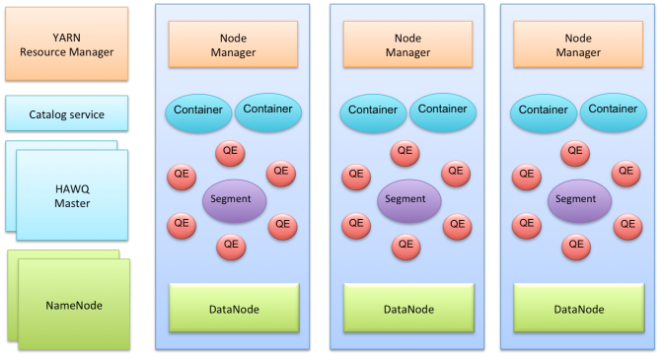
\includegraphics[width=\linewidth]{images/hawq-arch.png}}
	\caption{{The following diagram provides a high-level
	architectural view of a typical HAWQ
	deployment.}\cite{www-hawq-arch-image}.}
	\label{fig:false-color}
\end{figure}

\subsection{HAWQ Master}

The HAWQ master is the entry point to the system. It is the database
process that accepts client connections and processes the SQL
commands issued. The HAWQ master parses queries, optimizes queries,
dispatches queries to segments and coordinates the query execution.
End-users interact with HAWQ through the master and can connect to
the database using client programs such as psql or application
programming interfaces (APIs) such as JDBC \CE or ODBC \CE.The master is
where the global system catalog resides. The global system catalog is
the set of system tables that contain metadata about the HAWQ system
itself. The master does not contain any user data; data resides only
on HDFS.

\subsection{HAWQ Segment}

In HAWQ, the segments are the units that process data simultaneously.
There is only one physical segment on each host. Each segment can
start many Query Executors (QEs) for each query slice. This makes a
single segment act like multiple virtual segments, which enables HAWQ
to better utilize all available resources.

\subsection{HAWQ Interconnect}

The interconnect is the networking layer of HAWQ. When a user
connects to a database and issues a query, processes are created on
each segment to handle the query. The interconnect refers to the
inter-process communication between the segments, as well as the
network infrastructure on which this communication relies.

\subsection{HAWQ Resource Manager}

The HAWQ resource manager obtains resources from YARN and responds to
resource requests. Resources are buffered by the HAWQ resource
manager to support low latency queries. The HAWQ resource manager can
also run in standalone mode. In these deployments, HAWQ manages
resources by itself without YARN.

\subsection{HAWQ Catalog Service}

The HAWQ catalog service stores all metadata, such as
{UDF/UDT}\cite{www-udt}
information, relation information, security information and data file
locations.

\subsection{HAWQ Fault Tolerance Service}

The HAWQ fault tolerance service (FTS) is responsible for detecting
segment failures and accepting heartbeats from segments.

\subsection{HAWQ Dispatcher}

The HAWQ dispatcher dispatches query plans to a selected subset of
segments and coordinates the execution of the query. The dispatcher
and the HAWQ resource manager are the main components responsible for
the dynamic scheduling of queries and the resources required to
execute them.

\section{Key Features of Pivotal HDB/HAWQ}

\subsection{High-Performance Architecture}

Pivotal HDB’s parallel processing architecture delivers high
performance throughput and low latency (potentially, near-real-time)
query responses that can scale to petabyte-sized datasets. Pivotal
HDB also features a cutting-edge, cost-based SQL query optimizer and
dynamic pipelining technology for efficient performance operation.

\subsection{Robust ANSI SQL Compliance}

Pivotal HDB complies with ANSI SQL-92, -99, and -2003 standards, plus
OLAP extensions. \CE Leverage existing SQL expertise and existing
SQL-based applications and BI/data visualization tools. Execute
complex queries and joins, including roll-ups and nested queries.

\subsection{Deep Analytics and Machine Learning}

Pivotal HDB integrates statistical and machine learning capabilities
that can be natively invoked from SQL and applied natively to large
data sets across a Hadoop cluster. Pivotal HDB supports PL/Python,
PL/Java and PL/R programming languages.

\subsection{Flexible Data Format Support}

HDB supports multiple data file formats including Apache Parquet and
HDB binary data files, plus HBase and Avro via HDB’s Pivotal
Extension Framework (PXF) services. HDB interfaces with HCatalog,
which enables you to query an even broader range of data formats.

\subsection{Tight Integration with Hadoop Ecosystem}

Pivotal HDB plugs into the Apache Ambari  \CE installation, management and
configuration framework. This provides a Hadoop-native mechanism for
installation and deployment of Pivotal HDB and for monitoring cluster
resources across Pivotal HDB and the rest of the Hadoop ecosystem.

\section{Ecosystem}

HAWQ uses {Hadoop ecosystem}\cite{www-about-hadoop} integration and
manageability and flexible data-store format support. HAWQ is
natively in hadoop and requires no connectors.Hadoop Common contains
libraries and utilities needed by other Hadoop modules. HDFS is a
distributed file-system that stores data on commodity machines,
providing very high aggregate bandwidth across the cluster. Hadoop
YARN is a resource-management platform responsible for managing
computing resources in clusters and using them for scheduling of
users applications. Hadoop MapReduce is an implementation of the
MapReduce programming model for large scale data processing.

\section{Applications of Pivotal HD/HAWQ}

The Pivotal HD Enterprise product enables you to take advantage of
big data analytics without the overhead and complexity of a project
built from scratch. Pivotal HD Enterprise is Apache Hadoop that
allows users to write distributed processing applications for large
data sets across a cluster of commodity servers using a simple
programming model.

\subsection{Content-Based Image Retrieval using Pivotal HD with HAWQ}

Manual tagging is infeasible for image databases of this size, and is
prone to errors due to users’ subjective opinions.Given a query
image, a {CBIR}\cite{www-cbir} system can be potentially used to
auto-tag (label)
similar images in the collection, with the assigned label being the
object category or scene description label. This technology also has
an important role to play within a number of non-consumer domains.
CBIR systems can be used in health care contexts for case-based
diagnoses. A common example is {image retrieval on large image
databases such as Flickr}\cite{www-paper-cbir}.

\subsection{Transition of Hulu from Mysql to Pivotal-HD/HAWQ}

Hulu is a leading video company that offers TV shows, clips, movies
and more on the free, ad-supported Hulu.com service and the
subscription service Hulu Plus. It serves 4 billion videos. It has
used HAWQ to gain performance improvement to handle queries from
users. {It's main challenge was inability to scale MySQL and
Memcached to improve performance which was handled by Pivotal
HAWQ}\cite{www-pivotal-hulu}.


\section{Disadvantages}

There are also some drawbacks that needs attention before one choose to
use Pivotal-HD/HAWQ. Since most of these are used with the help
public cloud providers there is a greater dependency on service
providers,
Risk of being locked into proprietary or vendor-recommended systems,
Potential privacy and security risks of putting valuable data on someone else's system.
Another important problem what happens if the supplier suddenly stops
services. Even with this disadvantages the technology is still used
greatly in various industries and many more are looking forward to
move into cloud.

\section{Educational Material}

{Pivotal offers an portfolio of role-based courses and certifications
to build your product expertise}\cite{www-pivotal-courses}. These
courses can get someone with basic knowledge of hadoop ecosystem  to
understand how to deploy, manage, build, integrate and analyze
Pivotal HD/HAWQ applications on clouds.

\section{Conculsion}

Pivotal HD/HAWQ is the Apache Hadoop native SQL database for data
science and machine learning workloads. With Pivotal HDB we can ask
more questions on data in Hadoop to gain insights into data by using
all the available cloud resources without sampling data or moving it
into another platform for advanced analytics. Its fault tolerant
architecture can handle node failures and move the workload around
clusters.

\bibliography{references}
\TODO{Where is your bio?}
\end{document}
